\documentclass[12pt,a4paper,twoside]{article}

\textwidth 17cm \textheight 25cm \evensidemargin 0cm
\oddsidemargin 0cm \topmargin -2.5cm
\parindent 0pt
%\parskip \bigskipamount

\usepackage{graphicx}
\usepackage[dutch]{babel}
\usepackage{amssymb,amsthm,amsmath}
\usepackage[utf8]{inputenc}
\usepackage{nopageno}
\usepackage{pdfpages}
\usepackage{enumerate}
\usepackage{caption}
\usepackage{wrapfig}
\usepackage{pgf,tikz}
\usepackage{color}
\usetikzlibrary{arrows}
\usetikzlibrary{patterns}
\usepackage{fancyhdr}
\pagestyle{fancy}
\usepackage[version=3]{mhchem}
\usepackage{multicol}
\usepackage{fix-cm}
\usepackage{setspace}
\usepackage{mhchem}
\usepackage{xhfill}
\usepackage{parskip}
\usepackage{cancel}
\usepackage{mdframed}
\usepackage{url}

\newcommand{\todo}[1]{{\color{red} TODO: #1}}

\newcommand{\degree}{\ensuremath{^\circ}}
\newcommand\rad{\qopname\relax o{\mathrm{rad}}}

\newcommand\ggd{\qopname\relax o{\mathrm{ggd}}}

\def\LRA{\Leftrightarrow}%\mkern40mu}

\newcommand{\zrmbox}{\framebox{\phantom{EXE}}\phantom{X}}
\newcommand{\zrm}[1]{\framebox{#1}}

% environment oefening:
% houdt een teller bij die de oefeningen nummert, probeert ook de oefening op één pagina te houden
\newcounter{noefening}
\setcounter{noefening}{0}
\newenvironment{oefening}
{
  \stepcounter{noefening}
  \pagebreak[0]
  \begin{minipage}{\textwidth}
  \vspace*{0.7cm}{\large\bf Oefening \arabic{noefening}}
}{%
  \end{minipage}
}

\usepackage{calc}

% vraag
\reversemarginpar
\newcounter{punten}
\setcounter{punten}{0}
\newcounter{nvraag}
\setcounter{nvraag}{1}
\newlength{\puntwidth}
\newlength{\boxwidth}
\newcommand{\vraag}[1]{
\settowidth{\puntwidth}{\Large{#1}}
\setlength{\boxwidth}{1.5cm}
\addtolength{\boxwidth}{-\puntwidth}
{\large\bf Vraag \arabic{nvraag} \addtocounter{nvraag}{1}}\vspace*{-0.5cm}
{\marginpar{\color{lightgray}\fbox{\parbox{1.5cm}{\vspace*{1cm}\hspace*{\boxwidth}{\Large{#1}}}}}
\vspace*{0.5cm}}
\addtocounter{punten}{#1}}

% arulefill
\newcommand\arulefill[1][]{
  \ifstrempty{#1}{
    \leavevmode{
      \xrfill[-5pt]{0.3pt}[lightgray]
      \endgraf
    }
    \vspace*{0.2cm}
  }{
    \leavevmode{
      \xrfill[-5pt]{0.3pt}[lightgray]
      \endgraf
      \vspace*{0.2cm}
    }
    \foreach \n in {1,...,#1}{
      \leavevmode{
        \xrfill[-5pt]{0.3pt}[lightgray]
        \endgraf
        \vspace*{0.2cm}
      }
    }
  }
}
% \arules{n}
\newcommand{\arules}[1]{
\mbox{}
\color{lightgray}
%\vspace*{0.05cm}
\foreach \n in {1,...,#1}{
  \vspace*{0.75cm}
  \hrule height 0.3pt\hfill
}\color{black}\vspace*{0.2cm}}

% \arule{x}
\newcommand{\arule}[1]{
\color{lightgray}{\raisebox{-0.1cm}{\rule[-0.05cm]{#1}{0.3pt}}}\color{black}
}

% \abox{y}
\newcommand{\abox}[1]{
\fbox{
\begin{minipage}{\textwidth- 4\fboxsep}
\hspace*{\textwidth}\vspace{#1}
\end{minipage}
}
}

\newcommand{\ruitjes}[1]{
\definecolor{cqcqcq}{rgb}{0.85,0.85,0.85}
\hspace*{-2.5cm}
\begin{tikzpicture}[scale=1.04,line cap=round,line join=round,>=triangle 45,x=1.0cm,y=1.0cm]
\draw [color=cqcqcq, xstep=0.5cm, ystep=0.5cm] (0,-#1) grid (20.5,0);
\end{tikzpicture}
}


\newcommand{\assenstelsel}[5][1]{
\definecolor{cqcqcq}{rgb}{0.65,0.65,0.65}
\begin{tikzpicture}[scale=#1,line cap=round,line join=round,>=triangle 45,x=1.0cm,y=1.0cm]
\draw [color=cqcqcq,dash pattern=on 1pt off 1pt, xstep=1.0cm,ystep=1.0cm] (#2,#4) grid (#3,#5);
\draw[->,color=black] (#2,0) -- (#3,0);
\draw[shift={(1,0)},color=black] (0pt,2pt) -- (0pt,-2pt) node[below] {\footnotesize $1$};
\draw[color=black] (#3.25,0.07) node [anchor=south west] { x};
\draw[->,color=black] (0,#4) -- (0,#5);
\draw[shift={(0,1)},color=black] (2pt,0pt) -- (-2pt,0pt) node[left] {\footnotesize $1$};
\draw[color=black] (0.09,#5.25) node [anchor=west] { y};
\draw[color=black] (0pt,-10pt) node[right] {\footnotesize $0$};
\end{tikzpicture}
}

\newcommand{\getallenas}[3][1]{
\definecolor{cqcqcq}{rgb}{0.65,0.65,0.65}
\begin{tikzpicture}[scale=#1,line cap=round,line join=round,>=triangle 45,x=1.0cm,y=1.0cm]
\draw [color=cqcqcq,dash pattern=on 1pt off 1pt, xstep=1.0cm,ystep=1.0cm] (#2,-0.2) grid (#3,0.2);
\draw[->,color=black] (#2.25,0) -- (#3.5,0);
\draw[shift={(0,0)},color=black] (0pt,2pt) -- (0pt,-2pt) node[below] {\footnotesize $0$};
\draw[shift={(1,0)},color=black] (0pt,2pt) -- (0pt,-2pt) node[below] {\footnotesize $1$};
\draw[color=black] (#3.25,0.07) node [anchor=south west] {$\mathbb{R}$};
\end{tikzpicture}
}

\newcommand{\visgraad}[1]{\begin{tabular}{p{0.5cm}|p{#1}}&\\\hline\\\end{tabular}}

\newcommand{\tekenschema}[2]{\begin{tabular}{p{0.5cm}|p{#1}}&\\\hline\\[#2]\end{tabular}}

% schema van Horner
\newcommand{\schemahorner}{
\begin{tabular}{p{0.5cm}|p{7cm}}
&\\[1.5cm]
\hline\\
\end{tabular}}

% geef tabular iets meer ruimte
\setlength{\tabcolsep}{14pt}
\renewcommand{\arraystretch}{1.5}

\newcommand{\toets}[3]{
\thispagestyle{plain}
\vspace*{-2.5cm}
\begin{tikzpicture}[remember picture, overlay]
    \node [shift={(15.25 cm,-1.6cm)}] {%
        \includegraphics[width=1.8cm]{/home/ppareit/kaa1415/logokaavelgem.png}%
    };%
\end{tikzpicture}

\begin{tabular}{|llc|c|}
\hline
\vspace*{-0.5cm}
&&&\\
Naam & \arule{4cm} & {\Large\bf KA AVELGEM} & \\
\vspace*{-0.75cm}
&&&\\
Klas & \arule{4cm} & {\Large\bf 20...-...-...} & \\
\hline
\vspace*{-0.75cm}
&&&\\
Toets & {\bf #2} & {\large\bf #1} & Beoordeling\\
\vspace*{-0.75cm}
&&&\\
Onderwerp & \multicolumn{2}{l|}{\bf #3} &\\
\hline
\end{tabular}
}

\newcommand{\oefeningen}[1]{

\fancyhead[LE, RO]{\vspace{0.5cm} #1}
%\thispagestyle{plain}

{\bf \Large \centering Oefeningen: #1}

}

\raggedbottom

\newcommand\dom{\qopname\relax o{\mathrm{dom}}}
\newcommand\ber{\qopname\relax o{\mathrm{ber}}}

\newcommand\mC{\qopname\relax o{\mathrm{mC}}}
\newcommand\uC{\qopname\relax o{\mathrm{{\mu}C}}}
\newcommand\C{\qopname\relax o{\mathrm{C}}}

\newcommand\W{\qopname\relax o{\mathrm{W}}}
\newcommand\kW{\qopname\relax o{\mathrm{kW}}}
\newcommand\kWh{\qopname\relax o{\mathrm{kWh}}}


\newcommand\V{\qopname\relax o{\mathrm{V}}}
\newcommand\ohm{\qopname\relax o{\mathrm{\Omega}}}
\newcommand\kohm{\qopname\relax o{\mathrm{k\Omega}}}


\newcommand\N{\qopname\relax o{\mathrm{N}}}

\newcommand\Nperkg{\qopname\relax o{\mathrm{N/kg}}}

\newcommand\Nperm{\qopname\relax o{\mathrm{N/m}}}

\newcommand\gpermol{\qopname\relax o{\mathrm{g/mol}}}


\newcommand\kgperm{\qopname\relax o{\mathrm{kg/m}}}
\newcommand\kgperdm{\qopname\relax o{\mathrm{kg/dm}}}
\newcommand\gpercm{\qopname\relax o{\mathrm{g/cm}}}
\newcommand\gperml{\qopname\relax o{\mathrm{g/ml}}}


\newcommand{\mA}{\;\mbox{mA}}
\newcommand{\A}{\;\mbox{A}}
\newcommand{\MA}{\;\mbox{MA}}

\newcommand{\us}{\;\mu\mbox{s}}
\newcommand\s{\qopname\relax o{\mathrm{s}}}

\newcommand\h{\qopname\relax o{\mathrm{h}}}

\newcommand{\mpers}{\;\mbox{m/s}}
\newcommand{\kmperh}{\;\mbox{km/h}}
\newcommand{\kmpermin}{\;\mbox{km/min}}
\newcommand{\kmpers}{\;\mbox{km/s}}

\newcommand{\mph}{\;\mbox{mph}}

\newcommand{\Hz}{\;\mbox{Hz}}

\newcommand\Gm{\qopname\relax o{\mathrm{Gm}}}
\newcommand\Mm{\qopname\relax o{\mathrm{Mm}}}
\newcommand\km{\qopname\relax o{\mathrm{km}}}
\newcommand\hm{\qopname\relax o{\mathrm{hm}}}
\newcommand\dam{\qopname\relax o{\mathrm{dam}}}
\newcommand\m{\qopname\relax o{\mathrm{m}}}
\newcommand\dm{\qopname\relax o{\mathrm{dm}}}
\newcommand\cm{\qopname\relax o{\mathrm{cm}}}
\newcommand\mm{\qopname\relax o{\mathrm{mm}}}
\newcommand\um{\qopname\relax o{\mathrm{{\mu}m}}}
\newcommand\nm{\qopname\relax o{\mathrm{nm}}}


\newcommand\Gg{\qopname\relax o{\mathrm{Gg}}}
\newcommand\Mg{\qopname\relax o{\mathrm{Mg}}}
\newcommand\kg{\qopname\relax o{\mathrm{kg}}}
\newcommand\hg{\qopname\relax o{\mathrm{hg}}}
\renewcommand\dag{\qopname\relax o{\mathrm{dag}}}
\newcommand\g{\qopname\relax o{\mathrm{g}}}
\newcommand\dg{\qopname\relax o{\mathrm{dg}}}
\newcommand\cg{\qopname\relax o{\mathrm{cg}}}
\newcommand\mg{\qopname\relax o{\mathrm{mg}}}
\newcommand\ug{\qopname\relax o{\mathrm{{\mu}g}}}
\renewcommand\ng{\qopname\relax o{\mathrm{ng}}}

\newcommand\ton{\qopname\relax o{\mathrm{ton}}}

\newcommand\Gl{\qopname\relax o{\mathrm{Gl}}}
\newcommand\Ml{\qopname\relax o{\mathrm{Ml}}}
\newcommand\kl{\qopname\relax o{\mathrm{kl}}}
\newcommand\hl{\qopname\relax o{\mathrm{hl}}}
\newcommand\dal{\qopname\relax o{\mathrm{dal}}}
\renewcommand\l{\qopname\relax o{\mathrm{l}}}
\newcommand\dl{\qopname\relax o{\mathrm{dl}}}
\newcommand\cl{\qopname\relax o{\mathrm{cl}}}
\newcommand\ml{\qopname\relax o{\mathrm{ml}}}
\newcommand\ul{\qopname\relax o{\mathrm{{\mu}l}}}
\newcommand\nl{\qopname\relax o{\mathrm{nl}}}

\newcommand\MJ{\qopname\relax o{\mathrm{MJ}}}
\newcommand\kJ{\qopname\relax o{\mathrm{kJ}}}
\newcommand\J{\qopname\relax o{\mathrm{J}}}

\newcommand\T{\qopname\relax o{\mathrm{T}}}
\newcommand\uT{\qopname\relax o{\mathrm{{\mu}T}}}

\newcommand\grC{\qopname\relax o{\mathrm{{\degree}C}}}

\newcommand\K{\qopname\relax o{\mathrm{K}}}
\newcommand\calperK{\qopname\relax o{\mathrm{cal/K}}}

\newcommand\hPa{\qopname\relax o{\mathrm{hPa}}}
\newcommand\Pa{\qopname\relax o{\mathrm{Pa}}}

\newcommand\dB{\qopname\relax o{\mathrm{dB}}}

\newcommand{\EE}[1]{\cdot 10^{#1}}

\onehalfspacing

%\singlespacing
%\onehalfspacing
%\doublespacing

%\setlength{\headsep}{0cm}

\newenvironment{exlist}[1] %
{ \begin{multicols}{#1}
  \begin{enumerate}[(a)]
    \setlength{\itemsep}{0.8em} }
{ \end{enumerate}
  \end{multicols} }




\usepackage[outputdir=./build/]{dot2texi}
\usepackage{venndiagram}
\usepackage{makebox}
\usepackage{listings}

\newcommand{\dice}[1]{
\begin{tikzpicture}[x=1em,y=1em,radius=0.1]
  \draw[rounded corners=1] (0,0) rectangle (1,1);
  \ifodd#1
    \fill (0.5,0.5) circle;
  \fi
  \ifnum#1>1
    \fill (0.2,0.2) circle;
    \fill (0.8,0.8) circle;
   \ifnum#1>3
     \fill (0.2,0.8) circle;
     \fill (0.8,0.2) circle;
    \ifnum#1>5
      \fill (0.8,0.5) circle;
      \fill (0.2,0.5) circle;
    \fi
  \fi
\fi
\end{tikzpicture}
}

\begin{document}

\begin{center}
  \begin{mdframed}
  \centering
  \fontsize{40}{60}\selectfont Telproblemen
  \end{mdframed}
  \vfill
  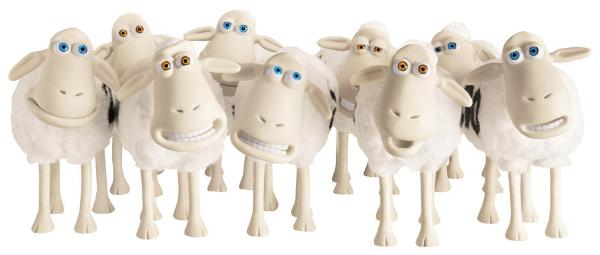
\includegraphics[width=\textwidth]{counting-sheep}
  \vfill
\end{center}
\subsection*{Doelstellingen}
{\singlespacing
Je kan \hfill  {\scriptsize(LP 2005-069, LI 2.1)}
\begin{itemize}
  \itemsep0em
  \item telproblemen oplossen waarbij de volgorde van de elementen van een groepering van belang is en herhaling van de elementen niet mogelijk.
  \item telproblemen oplossen waarbij de volgorde van de elementen van een groepering niet van belang is en herhaling van de elementen niet mogelijk.
\end{itemize}}

\thispagestyle{empty}
\clearpage

\tableofcontents
\thispagestyle{empty}
\clearpage

\pagenumbering{arabic}

\pagestyle{fancy}
\fancyhead[RO,LE]{Telproblemen}
\fancyhead[RE,LO]{}

We beginnen aan een hoofdstuk die vaak combinatoriek of combinatieleer wordt genoemd. Wij zullen voornamelijk problemen bespreken waarbij we het aantal mogelijkheden of het aantal objecten van een verzameling moeten tellen. We spreken dan ook van {\bf telproblemen}.

\section{Productregel}

\subsection{Voorbeeld}

Deze zomer ben ik eens op restaurant geweest en daar hing volgende menu:

\begin{center}
  \begin{minipage}{0.6\linewidth}
    \begin{mdframed}
      \begin{itemize}
      \item Voorgerechten:
        \begin{itemize}
        \item Garnaalkroketten
        \item Gerookte zalm
        \end{itemize}
      \item Hoofdgerechten:
        \begin{itemize}
        \item Lasagne
        \item Pasta met kip
        \item Biefstuk met pepersaus
        \end{itemize}
      \item Nagerechten:
        \begin{itemize}
        \item Appeltaart
        \item Sorbet
        \end{itemize}
      \end{itemize}
    \end{mdframed}
  \end{minipage}
\end{center}

Ik had uiteraard veel honger en bestelde één voorgerecht, één hoofdgerecht en één dessert.

We wensen dus een maaltijd samen te stellen, we nemen dus een {\bf samengestelde beslissing} gebaseerd op verschillende onafhankelijke deelbeslissingen in een willekeurige volgorde. Logisch is dat we eerst een voorgerecht kiezen, dan een hoofdgerecht en als laatste een dessert. Onze menu zal echter niet wijzigen als we eerst een beslissing nemen over het dessert en daarna over het voorgerecht en het hoofdgerecht.

De vraag is nu:\\
{\em Op hoeveel manieren kan ik mijn menu samenstellen?}

Om zeker te zijn dat we de telling juist doen zullen we het probleem grafisch gaan voorstellen. We kunnen dit op drie manieren doen, met een boomdiagram, met een wegendiagram of met een vaasmodel. Elke voorstellingswijze heeft voor- en nadelen.

\subsection{Boomdiagram}

\begin{adjustwidth}{-1.5cm}{-1.5cm}
\begin{dot2tex}[tikz, options=--tikzedgelabel]
  digraph G {
    node [shape=none,label=""];
    edge [arrowhead=none,lblstyle="above, sloped"];
    rankdir=LR;
    ranksep=0.3;
    a0 -> b0 [label="garnaal"];
    a0 -> b1 [label="zalm"];
    b0 -> c0 [label="lasagne"];
    b0 -> c1 [label="pasta"];
    b0 -> c2 [label="biefstuk"];
    b1 -> c3 [label="lasagne"];
    b1 -> c4 [label="pasta"];
    b1 -> c5 [label="biefstuk"];
    c0 -> d0 [label="taart"];
    c0 -> d1 [label="sorbet"];
    c1 -> d2 [label="taart"];
    c1 -> d3 [label="sorbet"];
    c2 -> d4 [label="taart"];
    c2 -> d5 [label="sorbet"];
    c3 -> d6 [label="taart"];
    c3 -> d7 [label="sorbet"];
    c4 -> d8 [label="taart"];
    c4 -> d9 [label="sorbet"];
    c5 -> d10 [label="taart"];
    c5 -> d11 [label="sorbet"];
    d0 [shape=none, label="ga,la,ta"]
    d1 [shape=none, label="ga,la,so"]
    d2 [shape=none, label="ga,pa,ta"]
    d3 [shape=none, label="ga,pa,so"]
    d4 [shape=none, label="ga,bi,ta"]
    d5 [shape=none, label="ga,bi,so"]
    d6 [shape=none, label="za,la,ta"]
    d7 [shape=none, label="za,la,so"]
    d8 [shape=none, label="za,pa,ta"]
    d9 [shape=none, label="za,pa,so"]
    d10 [shape=none, label="za,bi,ta"]
    d11 [shape=none, label="za,bi,so"]
    aa -> bb [style=dashed, label="Voorgerecht"];
    bb -> cc [style=dashed, label="Hoofdgerecht"];
    cc -> dd [style=dashed, label="Nagerecht"];
  }
\end{dot2tex}
\end{adjustwidth}

In een wiskundige boom worden de lijntjes de {\bf takken} genoemd. De takken komen steeds samen in de {\bf knopen}. De knoop waar begonnen wordt noemen we de {\bf wortel} en het eindpunten van de boom worden de {\bf bladen} genoemd.

In de bladen worden de mogelijke menu's opgeschreven. Zo hebben we bijvoorbeeld {\em ga,la,ta} voor garnaalkroketten als voorgerecht, lasagne als hoofdgerecht en appeltaart als dessert. We besluiten dat we eenvoudigweg het aantal mogelijke menu's kunnen bepalen door het aantal bladen te tellen.

\begin{oefening}
Neem eens de beslissingen in een andere volgorde, namelijk kies eerst een dessert, dan een voorgerecht en dan pas het hoofdgerecht. Teken de boom. Krijg je dezelfde boom? Krijg hetzelfde aantal mogelijkheden?
\end{oefening}

\subsection{Wegendiagram}

Een boomdiagram heeft als voornaamste nadeel dat deze heel snel heel groot wordt. Als je nu eens kijkt naar de boom, dan merk je dat er per beslissing evenveel takken vertrekken uit een knoop. Laat je de vertrekkende takken dus toekomen in eenzelfde knoop dan wordt de figuur veel compacter:

\begin{adjustwidth}{-1.5cm}{-1.5cm}
\begin{dot2tex}[tikz]
  digraph G {
    node [shape=none,label=""];
    edge [arrowhead=none];
    rankdir=LR;
    ranksep=0.55;
    a0 -> b0 [label="garnaal"];
    a0 -> b0 [label="zalm"];
    b0 -> c0 [label="lasagne"];
    b0 -> c0 [label="pasta"];
    b0 -> c0 [label="biefstuk"];
    c0 -> d0 [label="taart"];
    c0 -> d0 [label="sorbet"];
    aa -> bb [style=dashed, label="Voorgerecht"];
    bb -> cc [style=dashed, label="Hoofdgerecht"];
    cc -> dd [style=dashed, label="Nagerecht"];
  }
\end{dot2tex}
\end{adjustwidth}

Het tellen wordt nu moeilijker, we bekijken de verschillende deelbeslissingen apart.
\begin{itemize}
  \item Voor je voorgerecht neem je een eerste beslissing, je hebt $2$ keuzes.
  \item Voor je hoofdgerecht neem je een tweede beslissing, je hebt $3$ keuzes.
  \item Voor je dessert neem je een derde beslissing, je hebt $2$ keuzes.
\end{itemize}

We weten nu dat het aantal mogelijke menu's via de methode van het wegendiagram evenveel moet zijn als via de methode van het boomdiagram.

Het is dus evident dat we de keuzes bij elke deelbeslissing mogen vermenigvuldigen. Vandaar de productregel:
\begin{center}
  Het aantal mogelijke menu's is $2 \times 3 \times 2 = 12$
\end{center}

\subsection{Vaasmodel}

We kunnen het probleem ook voorstellen met behulp van vazen. Voor elke beslissing die we moeten nemen, nemen we een vaas met in deze vaas evenveel balletjes als het aantal keuzen die deze beslissing heeft.

\begin{multicols}{3}
  \begin{center}
    Voorgerecht
    \begin{tikzpicture}[scale=0.5,line cap=round,line join=round,>=triangle 45,x=1.0cm,y=1.0cm]
      \clip(-1.,-1.) rectangle (7.,3.);
      \draw [line width=1.6pt] (0.,2.)-- (0.,0.);
      \draw [line width=1.6pt] (0.,0.)-- (6.,0.);
      \draw [line width=1.6pt] (6.,0.)-- (6.,2.);
      \draw (1.1,1.8) node[anchor=north west] {ga};
      \draw (3.5,1.5) node[anchor=north west] {za};
    \end{tikzpicture}
  \end{center}
  \begin{center}
    Hoofdgerecht
    \begin{tikzpicture}[scale=0.5,line cap=round,line join=round,>=triangle 45,x=1.0cm,y=1.0cm]
      \clip(-1.,-1.) rectangle (7.,3.);
      \draw [line width=1.6pt] (0.,2.)-- (0.,0.);
      \draw [line width=1.6pt] (0.,0.)-- (6.,0.);
      \draw [line width=1.6pt] (6.,0.)-- (6.,2.);
      \draw (0.7,1.1) node[anchor=north west] {la};
      \draw (2.5,1.9) node[anchor=north west] {pa};
      \draw (3.8,1.0) node[anchor=north west] {bi};
    \end{tikzpicture}
  \end{center}
  \begin{center}
    Nagerecht
    \begin{tikzpicture}[scale=0.5,line cap=round,line join=round,>=triangle 45,x=1.0cm,y=1.0cm]
      \clip(-1.,-1.) rectangle (7.,3.);
      \draw [line width=1.6pt] (0.,2.)-- (0.,0.);
      \draw [line width=1.6pt] (0.,0.)-- (6.,0.);
      \draw [line width=1.6pt] (6.,0.)-- (6.,2.);
      \draw (1.1,1.2) node[anchor=north west] {ta};
      \draw (3.5,1.9) node[anchor=north west] {so};
    \end{tikzpicture}
  \end{center}
\end{multicols}

Je kan nu uit elke vaas een balletje nemen. Zo stel je bijvoorbeeld {\em ga,la,ta} samen. Dit kan je opnieuw doen, maar dan met andere keuzes. In het totaal kan je dat opnieuw 12 keer doen. Merk echter op dat we hier niet echt een formule krijgen waarbij we het totale aantal mogelijkheden vinden. Het vaasmodel verschaft ons echter wel inzicht in het telprobleem.

\subsection{Productregel}

Om een ander voorbeeld te bekijken: we wensen ons aan te kleden en we hebben keuze uit 3 truien en 2 broeken, dan kunnen we ons op $3 \cdot 2 = 6$ manieren kleden. Je kiest eerst een trui wat op 3 manieren kan, en bij elk van de drie keuzes van truien heb je twee mogelijkheden om een broek te kiezen. Dit soort telproblemen kunnen we oplossen met wat we de productregel noemen:

\paragraph*{Productregel}
\begin{mdframed}
Als een telprobleem bestaat uit $r$ onafhankelijke deelbeslissingen waarbij er voor de deelbeslissingen respectievelijk $n_1, n_2, \ldots , n_r$ mogelijkheden zijn, dan zijn er in het totaal
\[n_1 \cdot n_2 \cdot \ldots \cdot n_r\]
mogelijkheden.
\end{mdframed}

\needspace{4cm}
\subsection{Oefeningen}

\begin{oefening}
In een sportclub stelt men T-shirts, shorts en kousen ter beschikking voor de spelers. Er zijn oranje, witte, blauwe, rode en groene T-shirts. De shorts zijn zwart, blauw of wit. De kousen zijn wit met een blauwe boord ofwel effen wit. Er zijn dus heel wat outfits voor de spelers mogelijk.

Teken het boomdiagram en het wegendiagram dat met de gegevens correspondeert. Hoeveel mogelijke outfits zijn er voor de spelers?
\end{oefening}

\begin{oefening}
In de kantine van een fabriek staat een machine voor warme dranken. De leverancier wil gewone koffie, espresso en thee aanbieden, met of zonder melk, zonder, met weinig of met veel suiker. Hij heeft voor elke mogelijkheid een knop voorzien.

Teken het wegendiagram. Bepaal het aantal knoppen op de machine.
\end{oefening}

\begin{oefening}
Vanaf de ingang van de zoo zijn er drie paden naar het dolfinarium. Van het dolfinarium naar de apen zijn er 4 paden. Van de apen naar de pinguïns zijn er twee paden. En van de pinguïns naar de tijgers zijn er drie paden.\\
Ik wil naar de show van de dolfijnen gaan kijken. Als ik van de ingang naar de dolfijnen wandel zie ik de uren van de shows geafficheerd staan en merk ik dat ik nog ruim voldoende tijd heb om eerst een bezoekje te brengen aan de apen, de pinguïns en de tijgers.
\begin{enumerate}[(a)]
  \item Hoeveel verschillende wandelingen zijn er mogelijk van de ingang tot de tijgers?
  \item Bij de tijgers pauzeer ik even tot het tijd is om terug te keren naar het dolfinarium voor de show. Ik kies een wandeling terug via de pinguïns en de apen, maar wil een pad dat ik op de heenweg nam geen tweede keer bewandelen.\\
  Schets en wegendiagram van deze tweede wandeling. Hoeveel wandelingen zijn er nu mogelijk van de tijgers naar de dolfijnen?
\end{enumerate}
\begin{center}
  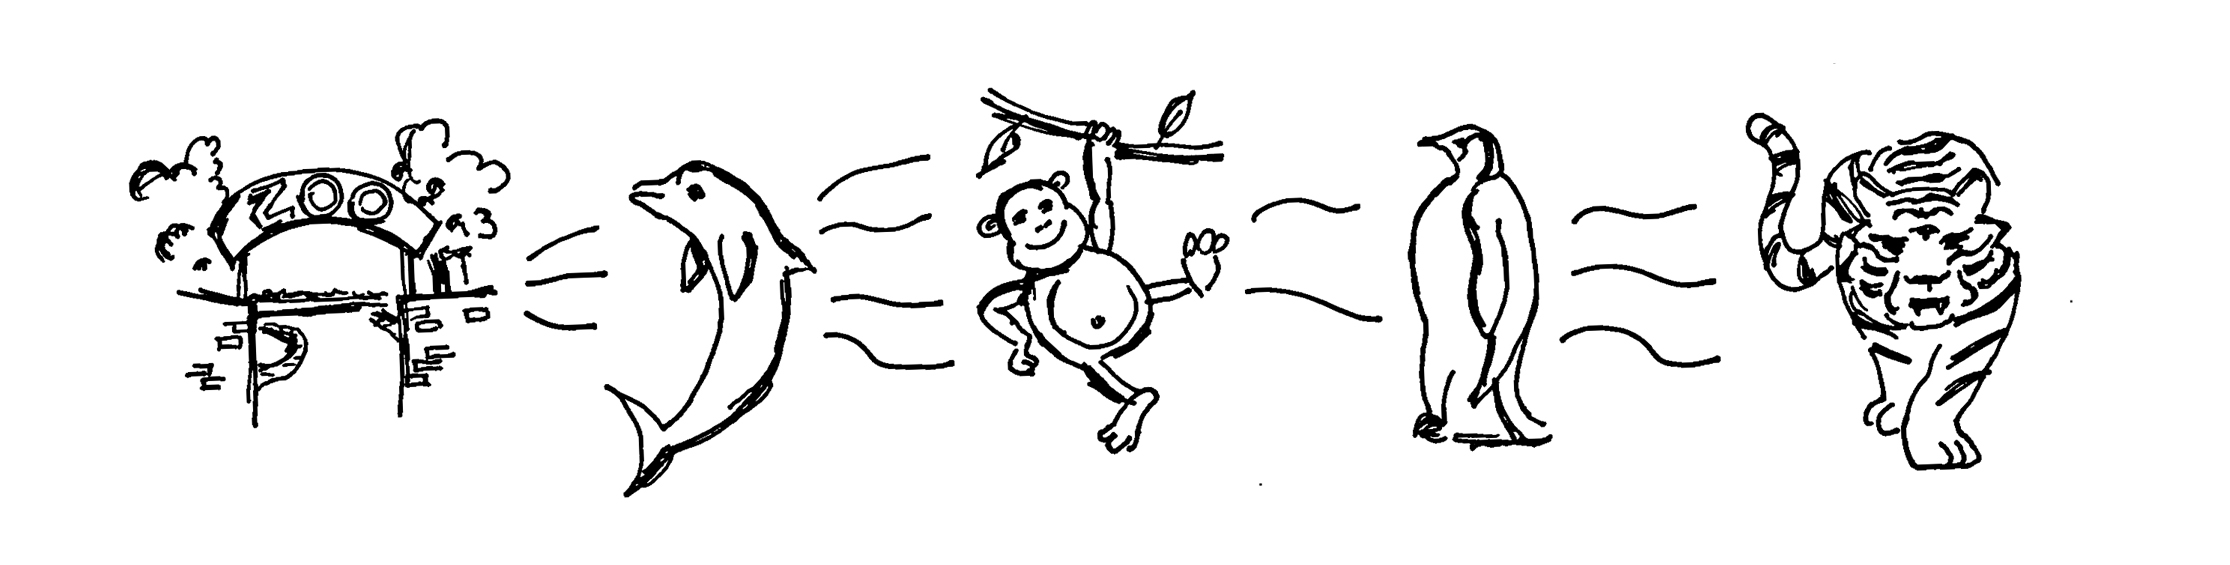
\includegraphics[width=\textwidth]{zoodieren}
\end{center}
\end{oefening}

\begin{oefening}
Los volgende problemen op met behulp van een boomdiagram.
\begin{enumerate}[(a)]
  \item Hoeveel natuurlijke getallen zijn er met drie cijfers, te kiezen uit 2, 3, 5 en 7?
  \item Hoeveel natuurlijke getallen zijn er met drie {\em verschillende} cijfers, te kiezen uit 2, 3, 5 en 7?
  \item Hoeveel natuurlijke getallen van drie verschillende cijfers, te kiezen uit 2, 3, 5 en 7, beginnen met een 5?
  \item Hoeveel natuurlijke getallen van drie verschillende cijfers, te kiezen uit 2, 3, 5 en 7, eindigen op een 5?
\end{enumerate}
\end{oefening}

\cleardoublepage
\section{Somregel}

\subsection{Somregel met dubbele telling}

\subsubsection*{Voorbeeld}

Vorige winter ben ik met een aantal vrienden uit het middelbaar iets gaan eten. We bestelden allemaal een hoofdgerecht en er werden 11 voorgerechten en 7 desserts besteld. Met vijf aten we zowel een voorgerecht als een dessert. Met hoeveel waren we?

Maak een venndiagram van de verzameling van de voorgerecht-eters en de nagerecht-eters. Leid hieruit het aantal af.

\begin{center}
\begin{venndiagram2sets}[labelOnlyA={$6$}, labelOnlyB={$2$}, labelAB={$5$}, labelNotAB={$\geq 0$}]
  \setpostvennhook{
    \draw[<-] (labelA) --++(120:1.6) node[above]{Voorgerecht (en hoofdgerecht)};
    \draw[<-] (labelB) --++(50:1.5) node[right]{Nagerecht (en hoofdgerecht)};
    \draw[<-] (labelAB) --++(-20:2.8) node[right, text width=4.5cm]{Voorgerecht en nagerecht (en hoofdgerecht)};
    \draw[<-] (labelNotAB) --++(-120:0.8) node[left]{Enkel hoofdgerecht};
  }
\end{venndiagram2sets}
\end{center}
Als je dus het aantal personen met een dessert het aantal personen met een voorgerecht optelt dan tel je de personen die een voorgerecht en een dessert hebben gegeten dubbel. Je kan dit compenseren door door eenmaal de personen die je dubbel hebt geteld er weer van af te trekken.

\paragraph*{Somregel}
\begin{mdframed}
Voor het aantal elementen van de unie van twee verzamelingen $A$ en $B$ geldt:
$$\#(A \cup B) = \#A + \#B - \#(A \cap B)$$
waarin
\begin{itemize}
  \item $\#A$ staat voor het aantal elementen van de verzameling $A$
  \item $A\cup B$ staat voor de unie (vereniging) van de verzamelingen $A$ en $B$, we kunnen dit ook omschrijven als $A$ {\em of} $B$
  \item $A\cap B$ staat voor de doorsnede van de verzamelingen $A$ en $B$, we kunnen dit ook omschrijven als $A$ {\em en} $B$
\end{itemize}
\end{mdframed}

\begin{oefening}
Bepaal met behulp van de somregel het aantal kaarten in een set van 52 kaarten die harten of koning zijn. Gebruik een set kaarten om dit te controleren. Maak ook een het bijhorende venndiagram.
\end{oefening}

\subsection{Somregel van elkaar uitsluitende mogelijkheden}

\subsubsection*{Voorbeeld}

Bepaal het aantal natuurlijke getallen van vier verschillende cijfers die deelbaar zijn door 5.

Om inzicht te krijgen in het probleem beginnen we met een aantal voorbeelden op te schrijven:
\begin{center}
  \texttt{1235} \qquad \texttt{2345} \qquad \texttt{1250} \\
  \texttt{\cancel{5023}} \qquad \texttt{6520} \qquad \texttt{\cancel{6500}}
\end{center}

We merken dat de getallen die we zoeken steeds eindigen op $0$ of op $5$. We gebruiken deze eigenschap om twee verzamelingen te maken:
\begin{itemize}
\item $A$: verzameling van alle getallen bestaande uit 4 verschillende cijfers die eindigen op $0$
\item $B$: verzameling van alle getallen bestaande uit 4 verschillende cijfers die eindigen op $5$
\end{itemize}

\begin{center}
  \begin{venndiagram2sets}
    [labelOnlyA={\scalebox{0.5}{$\ub\ub\ub\ub[0]$}},
    labelOnlyB={\scalebox{0.5}{$\ub\ub\ub\ub[5]$}}]
    \fillACapB
  \end{venndiagram2sets}
\end{center}

We merken dat de doorsnede ledig is:
$$A \cap B = \emptyset$$

We zeggen dat de deelverzamelingen elkaar {\bf uitsluitende mogelijkheden} zijn. Dit wil zeggen dat we de somregel kunnen toepassen zonder dat we het aantal elementen in de doorsnede moeten uitrekenen.

\begin{align*}
\#A &= 9 \cdot 8 \cdot 7 \cdot 1 = 504\\
\#B &= 8 \cdot 8 \cdot 7 \cdot 1 = 448\\
\Rightarrow \#(A \cup B) &= 504 + 448 = 952
\end{align*}

\paragraph*{Somregel voor elkaar uitsluitende mogelijkheden}
\begin{mdframed}
Zijn de twee verzamelingen $A$ en $B$ elkaar uitsluitende mogelijkheden omdat ze geen elementen gemeenschappelijk hebben, dan geldt voor het aantal elementen in hun unie:
\[\#(A\cup B) = \#A + \#B\]
\end{mdframed}

\begin{oefening}
Een club bestaat uit 30 mannelijke en 50 vrouwelijke leden.
\begin{enumerate}[(a)]
  \item Op hoeveel manieren kan men 1 lid kiezen als voorzitter?
  \item Op hoeveel manieren kan men 1 mannelijk en 1 vrouwelijk lid kiezen als bestuurslid?
\end{enumerate}
\end{oefening}

\begin{oefening}
In een bibliotheek zijn 50 wetenschappelijke verhandelingen, 100 detectiveverhalen en 180 romans beschikbaar. Op hoeveel manieren kan men hieruit 1 boek kiezen? Op hoeveel manieren kan iemand een lijstje opstellen met 1 boek van elke soort?
\end{oefening}

\subsection{Praktisch}

\begin{mdframed}
Bij het oplossen van telproblemen tel je als volgt:
\begin{itemize}
  \item Kan je een boomdiagram maken, dan is het aantal mogelijkheden gelijk aan het aantal bladen.
  \item Kan je een wegendiagram maken, dan is het aantal mogelijkheden gelijk aan het product van de keuzes bij elke beslissing.
  \item Kan je een probleem herschrijven met behulp van {\bf EN}, dan gebruik je de productregel.
  \item Kan je een probleem herschrijven met behulp van {\bf OF}, dan gebruik je de somregel.
\end{itemize}
\end{mdframed}

Hint: Maak steeds een het vaasmodel om inzicht te krijgen in het probleem.

\needspace{4cm}
\subsection{Oefeningen}

\begin{oefening}\\
\begin{minipage}[]{0.7\textwidth}
We moeten de afloop van 10 voetbalwedstrijden voorspellen. Voor elke match zijn er 3 mogelijkheden: winnen, verliezen en gelijkspel. Hoeveel lijstjes met voorspellingen zijn er mogelijk? Hoe groot is het aantal als we zeker weten dat in de eerste wedstrijd de thuisploeg niet verliest?
\end{minipage}
\begin{minipage}[]{0.29\textwidth}
  \centering
  
\includegraphics[width=0.5\textwidth]{voetbal}
\end{minipage}
\end{oefening}

\begin{oefening}
Voor de samenstelling van je lessenrooster moet je twee keuzevakken kiezen, elk uit een verschillend vakgebied. Er is keuze uit 3 talen, 4 wetenschappelijke vakken en 2 sporten. Hoeveel keuzemogelijkheden heb je?
\end{oefening}

\begin{oefening}
Het letterslot van een kluis bestaat uit een eerste ring met 10 letters, een tweede ring met 8 letters en een derde ring met 6 letters. Om een kluis te openen moet elke ring zo geplaatst worden dat een bepaalde stand inneemt.
\begin{enumerate}[(a)]
  \item Hoeveel lettergroepen moet een inbreker ten hoogste proberen?
  \item Hoeveel zijn er mogelijk als hij weet dat de letter van de eerste ring een E is?
\end{enumerate}
\end{oefening}

\begin{oefening}
Bij een schoolwedstrijd met 2 ploegen, die elk uit 6 deelnemers bestaan, moet elke deelnemer van de ene ploeg tegen elke deelnemer van de andere ploeg 2 partijen spelen. Hoeveel partijen zijn er in totaal?
\end{oefening}

\begin{oefening}
Bij de aankoop van een wagen moeten we kiezen tussen modellen met 2, 3, 4 of 5 deuren. De wagens met 2 of 3 deuren worden afgeleverd met een motor van 1200, 1400, 1600 of 1800 cc en de wagens met 4 of 5 deuren worden afgeleverd met een motor van 1600, 1800 of 2000 cc. Elke wagen is beschikbaar in 8 kleuren, maar voor de versies 1800 en 2000 cc zijn er bovendien nog 4 gemetalliseerde kleuren mogelijk. Voor wagens met een motor van 1200 cc bestaat er maar 1 type banden, wagens met een grotere motor kunnen naar keuze met één van 2 types banden worden uitgerust. Alle versies zijn verkrijgbaar met of zonder radio. Hoeveel mogelijkheden hebben we bij deze aankoop?
\end{oefening}

\begin{oefening}
Je hebt gewonnen op de foor. Je mag twee prijzen kiezen. Je mag kiezen uit drie verschillende tonnen. Je mag geen twee prijzen kiezen uit dezelfde ton. De eerste ton bevat 3 verschillende mp3-spelers. De tweede ton bevat 4 verschillende sleutelhangers. De laatste ton bevat 2 verschillende horloges. Hoeveel mogelijkheden om te kiezen heb je?
\end{oefening}

\begin{oefening}
Konijnenrassen bestaan in drie soorten: dwergkonijnen, gewone konijnen of reuze konijnen. Alle rassen komen voor als zwart, bruin of wit. Het gewone konijn komt ook nog voor in een zwart-bruin-wit gevlekte variant. Naast de rechtopstaande oren die we gewoon zijn van de konijnen komen dwerg en reuze konijnen ook voor met hangoren. Hoeveel mogelijke soorten konijnen bestaan er dan?
\end{oefening}

\begin{oefening}
Met de cijfers $1, 2, 3, \ldots , 8, 9$ worden getallen van 6 verschillende cijfers gevormd:
\begin{enumerate}[(a)]
  \item Hoeveel zulke getallen zijn er?
  \item Hoeveel van deze getallen beginnen met een 1?
  \item Hoeveel van deze getallen beginnen niet met een 5?
  \item Hoeveel van deze getallen beginnen met 55?
  \item Hoeveel van deze getallen bevatten een 4?
  \item Hoeveel van deze getallen bevatten een 3 en een 8?
  \item Hoeveel van deze getallen bevatten geen 3 en geen 8?
\end{enumerate}
\end{oefening}

\begin{oefening}
Ik ben de pincode van mijn GSM vergeten. Ik weet enkel nog dat er geen 5 in komt, maar wel een 4, en dat het allemaal verschillende cijfers waren. Hoeveel keer moet ik ten hoogste proberen om mijn code terug te vinden (in de veronderstelling dat je zoveel mag proberen als je wilt, zonder dat je sim-kaart geblokkeerd wordt)?
\end{oefening}

\begin{oefening}
Stel een boomdiagram op voor de natuurlijke getallen, bestaande uit drie verschillende cijfers, die je met 0, 1, 2, 3 en 4 kan vormen. Hoeveel mogelijke getallen zijn er?
\end{oefening}

\begin{oefening}
Hoeveel getallen, gevormd met de cijfers 0, 5, 6 en 8, liggen tussen 5000 en 6000 (deze twee uitersten inbegrepen) als een cijfer geen tweede maal mag gebruikt worden? Verduidelijk je antwoord met een boomdiagram.
\end{oefening}

\begin{oefening}
Je moet een menu opstellen. Hierbij moet er keuze zijn tussen 2 voorgerechten en 3 hoofdgerechten voor de {\em vegetariërs} en 3 voorgerechten en 4 hoofdgerechten voor de {\em alleseters}. Voor {\em iedereen} is er keuze uit 2 desserts. Hoeveel mogelijke menu's kan je samenstellen?
\end{oefening}

\cleardoublepage
\section{Variaties}

\subsection{Voorbeeld}

Op hoeveel manieren kunnen vier verschillende bollen in zes verschillende vakjes geplaatst worden? In elk vakje mag hoogstens één bol voorkomen.

We definiëren:
\begin{itemize}
  \item De verzameling bollen = $\{ \ast, \star, \circ, \bullet \}$
  \item De verzameling vakjes = $\{ \ub_a, \ub_b, \ub_c, \ub_d, \ub_e, \ub_f\}=\{a,b,c,d,e,f\}$
\end{itemize}

Een aantal voorbeelden van plaatsingen zijn
\[\ub[\ast]_a\ub[\star]_b\ub[\circ]_c\ub[\bullet]_d\ub_e\ub_f \qquad \ub_a\ub[\ast]_b\ub[\star]_c\ub[\circ]_d\ub[\bullet]_e\ub_f \]
\[\cancel{\ub[\ast]_a\ub[\ast]_b\ub[\ast]_c\ub[\ast]_d\ub_e\ub_f} \qquad \ub_a\ub[\bullet]_b\ub[\circ]_c\ub[\star]_d\ub[\ast]_e\ub_f \]
\[\ub[\ast]_a\ub_b\ub[\circ]_c\ub_d\ub[\bullet]_e\ub[\star]_f \qquad \cancel{\ub[\Overset{\bullet}{\circ}]_a\ub[\ast]_b\ub[\star]_c\ub_d\ub_e\ub_f} \]

Het is duidelijk dat elke plaatsing bestaat uit het nemen van $4$ deelbeslissingen. Namelijk, kiezen waar we eerst $\ast$ plaatsen, dan kiezen waar we $\star$ plaatsen, dan kiezen waar we $\circ$ plaatsen en uiteindelijk kiezen waar we $\bullet$ plaatsen. Om de plaatsing
\[\ub[\ast]_a\ub_b\ub[\circ]_c\ub_d\ub[\bullet]_e\ub[\star]_f\]
te krijgen, worden volgende vakjes gekozen:
\[a, f, c, e\]

Merk op dat het wijzigen van de volgorde, namelijk $a, c, e, f$ ons een andere plaatsing geeft. We zeggen dat de volgorde van belang is. Merk ook op dat er in elk vakje hoogstens één bol mag liggen of ook dat elke bol maar in hoogstens één vakje mag liggen. We zeggen dat herhaling niet toegestaan is.

Elk viertal is een samengestelde beslissing zonder herhaling. Wel, zulk viertal
noemt men een variatie zonder herhaling, kortweg variatie van vier verschillende bollen gekozen uit zes verschillende vakjes.

Het aantal variaties kunnen we nu gemakkelijk vinden als we de productregel gebruiken. Het aantal variaties van 4 elementen uit 6 elementen schrijven we kort met het nieuwe symbool $V^4_6$. We vinden dus
\[ V^4_6 = 6 \cdot 5 \cdot 4 \cdot 3 = 360 \]

\subsection{Formule}

\paragraph*{Stelling}
\begin{mdframed}
Het aantal {\bf variaties van $k$ verschillende elementen gekozen uit $n$ verschillende elementen} noteren we $V^k_n$ en er geldt:
$$V^k_n=n \cdot (n-1) \cdot (n-2) \cdots (n-k+1)$$
\end{mdframed}

\paragraph*{Bewijs}
Er worden $k$ elementen gekozen. We nemen dus $k$ deelbeslissingen:
\begin{center}
\begin{tabular}{lp{12cm}}
$1$-ste beslissing: & We kunnen kiezen uit $n$ verschillende elementen\\
$2$-de beslissing: & We kunnen maar niet meer kiezen uit $n-1$ verschilende elementen meer want bij een variatie is herhaling niet toegestaan.\\
$\vdots$ & \\
$k$-de beslissing: & Er zijn nog $n-(k-1)=n-k+1$ elementen over om uit te kiezen.
\end{tabular}
\end{center}
Daar elke beslissing moet worden genomen, kunnen we elke beslissing verbinden met een '{\bf en}'. Met de productregel volgt dus de stelling.


\paragraph*{Opmerking} Er zal steeds gelden dat $k\leq n$.

\paragraph*{Belangrijk}
\begin{itemize}
  \item De positie waarin de elementen worden geplaatst is belangrijk, {\bf volgorde is van belang}.
  \item De elementen kunnen maar éénmaal worden gebruikt, {\bf herhaling is niet mogelijk}.
\end{itemize}

\begin{oefening}
Bereken:
\begin{multicols}{3}
\begin{enumerate}[(a)]
  \item $V^3_5$
  \item $V^2_7$
  \item $V^4_4$
\end{enumerate}
\end{multicols}
\end{oefening}

\begin{oefening}
\begin{enumerate}[(a)]
  \item Hoeveel variaties zijn er van $5$ elementen gekozen uit $8$ elementen?
  \item Hoeveel variaties zijn er als we $7$ keuzes hebben en we moeten $2$ elementen kiezen?
  \item Waarom kunnen we de $V^4_2$ niet uitrekenen?
  \end{enumerate}
\end{oefening}

\subsection{Bijzonder geval}

Voor $k=n$ wordt de formule
\[V^n_n = n \cdot (n-1) \cdot (n-2) \cdots 3 \cdot 2 \cdot 1\]

Het product van de opeenvolgende natuurlijke getallen van $1$ t.e.m. $n$ noteren we met $n!$ en we zeggen $n$-faculteit. We komen hier later nog op terug.

Omdat dit vaak voorkomt zullen we hier een naam aan geven, we spreken van {\bf de permutaties van $n$ elementen}. Dus een permutatie is een variatie van alle $n$ elementen uit $n$.

\paragraph*{Notatie:} $P_n = n! = n \cdot (n-1) \cdot (n-2) \cdots 3 \cdot 2 \cdot 1$

\begin{oefening}
\begin{enumerate}[(a)]
  \item Wat is het aantal variaties van 5 elementen gekozen uit 5 elementen?
  \item Hoeveel permutaties van 7 elementen zijn er?
\end{enumerate}
\end{oefening}

\subsection{Oefeningen}

\begin{minipage}{0.7\textwidth}
\begin{oefening}
Hiernaast zie je een vlag die ontworpen is voor een sportclub. Aan de jongste leden wordt gevraagd elk van de drie gebieden met een andere kleur te vullen.
\begin{enumerate}[(a)]
  \item Bert neemt een doos met 12 kleurpotloden. Hoeveel verschillende vlaggen kan hij produceren?
  \item Sara kiest voor de kleuren geel, oranje en blauw. Hoeveel verschillende vlaggen kan zij maken?
\end{enumerate}
\end{oefening}
\end{minipage}
\begin{minipage}{0.25\textwidth}
\begin{tikzpicture}[scale=0.3,line cap=round,line join=round,>=triangle 45,x=1.0cm,y=1.0cm]
\clip(-3,-3) rectangle (13,7);
\draw [line width=1.2pt] (-2,6)-- (-2,-2);
\draw [line width=1.2pt] (-2,-2)-- (12,-2);
\draw [line width=1.2pt] (12,-2)-- (12,6);
\draw [line width=1.2pt] (12,6)-- (-2,6);
\draw [line width=1.2pt] (8,2) circle (2cm);
\draw [line width=1.2pt] (10,2)-- (12,2);
\draw [line width=1.2pt] (6,2)-- (-2,2);
\end{tikzpicture}
\end{minipage}

\begin{oefening}
Op het {\em todo}-lijstje van Jef staan zeven dringende taken en vier niet dringende.
\begin{enumerate}[(a)]
  \item Hij neemt zijn agenda en noteert op elke dag van van volgende week één van de dringende taken. Op hoeveel manieren kan hij zijn agenda voor die week invullen?
  \item Als hij geen rekening houdt met de dringendheid van de taken, op hoeveel manieren kan hij dan zijn werk verdelen over de volgende week? Hij wil nog steeds maar één taak per dag uitvoeren.
  \item Eén van de dringende zaken wil hij per se op zaterdag uitvoeren en één van de niet dringende op zondag. Op hoeveel manieren kan hij nu zijn agenda invullen als hij weer uit de volledige lijst kiest?
\end{enumerate}
\end{oefening}

\begin{oefening}
Aan een paardenkoers nemen 8 paarden deel. Er wordt gevraagd de eerste 4 paarden in de juiste volgorde te geven. Hoeveel van dergelijke voorspellingen zijn er mogelijk?
\end{oefening}

\begin{oefening}
Een jeugdgroep telt 10 leden en wil een bestuur kiezen bestaande uit een voorzitter, een ondervoorzitter, een secretaris en een penningmeester. Hoeveel verschillende bestuurslichamen kunnen er verkozen worden?
\end{oefening}

\begin{oefening}
Op een boekenrek moeten 3 werken over wiskunde en 4 romans gerangschikt worden. We beschikken daartoe over 5 wiskundeboeken en over 6 romans. Op hoeveel manieren kunnen we de boeken rangschikken als ons opgelegd wordt de wiskundeboeken vooraan te plaatsen?
\end{oefening}

\begin{oefening}
Met de cijfers $1, 2, 3, \ldots, 9$ vormen we getallen van $6$ verschillende cijfers.
\begin{enumerate}[(a)]
  \item Hoeveel dergelijke getallen zijn er?
  \item Hoeveel ervan beginnen met 1?
  \item Hoeveel ervan beginnen niet met 2?
  \item Hoeveel ervan beginnen met 83?
  \item Hoeveel ervan beginnen niet met 123?
  \item Hoeveel ervan bevatten het cijfer 7?
  \item Hoeveel ervan bevatten wel 4, maar niet 5?
  \item Hoeveel ervan bevatten noch 8, noch 9?
  \item Hoeveel ervan bevatten de cijfers 4 en 5?
\end{enumerate}
\end{oefening}

\begin{oefening}
Op hoeveel manieren kan ik 10 boeken op een plank rangschikken als een bepaald boek op de eerste plaats moet staan?
\end{oefening}

\begin{oefening}
Op hoeveel manieren kunnen we 4 jongens en 3 meisjes op een rij zetten als in geen geval 2 jongens naast elkaar mogen staan?
\end{oefening}

\begin{oefening}
\begin{enumerate}[(a)]
  \item Schrijf alle permutaties van de elementen $a,b,c,d$ op.
  \item Schrijf alle permutaties van de elementen $a,b,c,c$ op.
\end{enumerate}
\end{oefening}

\begin{oefening}
We moeten vijf verschillende prijzen verloten onder de nummers 1 tot en met 100.
Het eerste getrokken nummer krijgt de mooiste prijs, enz. Na het trekken wordt het
nummer verwijderd (We spreken van trekken zonder terugleggen.)
Geef het aantal mogelijke trekkingen.
\end{oefening}

\begin{oefening}
Een vlag moet bestaan uit 2 verticale banen van verschillend gekleurde stof.
Men beschikt over 8 kleuren. Hoeveel vlaggen zijn hiermee samen te stellen?
\end{oefening}

\begin{oefening}
Met de cijfers $3, 4, 5, 6, 7, 8$ worden getallen van $3$ verschillende cijfers gevormd.
\begin{enumerate}[(a)]
  \item Hoeveel dergelijke getallen bestaan er?
  \item Hoeveel van deze getallen eindigen op $5$?
\end{enumerate}
\end{oefening}

\cleardoublepage
\section{Herhalingsvariaties}

\subsection{Voorbeeld}

Op hoeveel manieren kunnen vijf, verschillend gekleurde bollen in 3 vakjes geplaatst worden? In elk vakje is er plaats voor méér dan één bol.

We definieren de verzameling van bollen en verzameling vakjes voor het probleem:

\begin{itemize}
\item bollen = $\{ \oplus, \ominus, \otimes, \oslash, \odot \}$
\item vakjes = $\{ \ubx_a, \ubx_b, \ubx_c \} = \{ a, b, c\}$
\end{itemize}

Een aantal voorbeeldplaatsingen zijn
\[ \ubx[\oplus\ominus\otimes\oslash\odot]_a\ubx_b\ubx_c \qquad \ubx[\oplus\otimes\ominus]_a\ubx_b\ubx[\odot\oslash]_c\]
\[ \cancel{\ubx[\oplus\oplus]_a\ubx_b\ubx_c} \qquad \ubx[\oplus\ominus]_a\ubx_b\ubx[\odot\oslash\otimes]_c\]
\[ \ubx[\oplus]_a\ubx[\ominus]_b\ubx[\otimes\oslash\odot]_c=\ubx[\oplus]_a\ub[\ominus]_b\ubx[\odot\oslash\otimes]_c \]

De manier van bollen plaatsen is een samengestelde beslissing bestaande uit $5$ deelbeslissingen. Plaatsen we $\oplus, \ominus, \otimes, \oslash, \odot$ in die volgorde om de volgende plaatsing te verkrijgen
\[\ubx[\otimes\oslash]_a\ubx[\ominus]_b\ubx[\oplus\odot]_c\]
dan kiezen we de volgende vakjes
\[c, b, a, a, c\]

Merk ook hier op dat het wijzigen van de volgorde, bijvoorbeeld $a, a, b, c, c$ ons een totaal andere plaatsing geeft. Opnieuw krijgen we een probleem waarbij de volgorde van belang is. Bij dit probleem kan het wel dat er in een vakje meer dan één bol mag liggen. We zeggen dat herhaling toegestaann is.

Elk vijftal is een samengestelde beslissing met herhaling. Wel, zulk vijftal noemen we een herhalingsvariatie van vijf elementen gekozen uit een totaal van drie elementen. Het aantal herhalingsvariaties kunnen we nu gemakkelijk vinden als we de productregel gebruiken. Het aantal herhalingsvariaties van 5 elementen uit 3 elementen schrijven we kort met het nieuwe symbool $\bar{V}^5_3$. We vinden dus
\[\bar{V}^5_3 = 3 \cdot 3 \cdot 3 = 3^5 = 243\]

\paragraph*{Let op de notatie}
De $\bar{V}$ is het symbool voor het aantal herhalingsvariaties. Het aantal deelbeslissingen (bollen leggen) wordt bovenaan genoteerd. Het aantal keuzes (vakjes) wordt onderaan als index geschreven.

\subsection{Formule}

\paragraph*{Stelling}
\begin{mdframed}
Het aantal {\bf herhalingsvariaties van $k$ verschillende elementen gekozen uit $n$ verschillende elementen} noteren we $\bar{V}^k_n$ en er geldt:
$$\bar{V}^k_n=n^k$$
\end{mdframed}

\paragraph*{Bewijs} Het bewijs verloopt analoog als het bewijs van de formule voor gewone variaties. Met het verschil natuurlijk dat herhaling nu wel mag. Doe dit bewijs als oefening.

\paragraph*{Belangrijk}
\begin{itemize}
  \item De positie waarin de elementen worden geplaatst is belangrijk, {\bf volgorde is van belang}.
  \item De elementen kunnen meer dan eens op de zelfde positie terecht komen, {\bf herhaling is mogelijk}.
\end{itemize}

\subsection{Oefeningen}

\begin{oefening}
Aline, Birgit, Celine en Delphine zijn leerlingen uit eenzelfde klas die alle vier in de maand april verjaren.
\begin{enumerate}[(a)]
  \item Hoeveel mogelijkheden zijn er voor hun vier verjaardagen?
  \item Hoeveel mogelijkheden zijn er als je weet dat het vier verschillende data zijn?
  \item Als je weet dat Celine op 10 april jarig is, hoeveel mogelijkheden zijn er dan voor de vier verjaardagen als ze niet noodzakelijk op een verschillende dag moeten verjaren?
\end{enumerate}
\end{oefening}

\begin{oefening}
Met de cijfers 1, 2 en 3 worden getallen van 5 cijfers gevormd.
\begin{enumerate}[(a)]
  \item Hoeveel getallen zijn er?
  \item Hoeveel van die getallen zijn even?
  \item Hoeveel van die getallen bevatten geen cijfer 1?
  \item Hoeveel van die getallen bestaan uit 5 verschillende cijfers?
  \item Welk getal staat op de vijfde plaats als je alle getallen van klein naar groot rangschikt?
\end{enumerate}
\end{oefening}

\begin{oefening}
Bij een gezelschapsspel moeten we 4 gekleurde staafjes in een zekere volgorde naast elkaar zetten. Hoeveel mogelijkheden zijn er als we over 6 kleuren beschikken? Je mag er van uit gaan dat elk kleur voldoende voorradig is.
\end{oefening}

\begin{oefening}
Een leraar moet zijn leerlingen evalueren door achter hun naam één van de vermeldingen uitstekend (U), zeer goed (ZG), goed (G), voldoende (V), niet voldoende (NV) of slecht (S) te schrijven. Op hoeveel manieren kan hij een lijst van 12 leerlingen invullen?
\end{oefening}

\begin{oefening}
Van 1962 tot 1971 hadden kentekenplaten twee aaneengeschakelde letters en daarna 3 cijfers in willekeurige volgorde. Hoeveel mogelijke nummerplaten konden ze toen maken?
\begin{center}
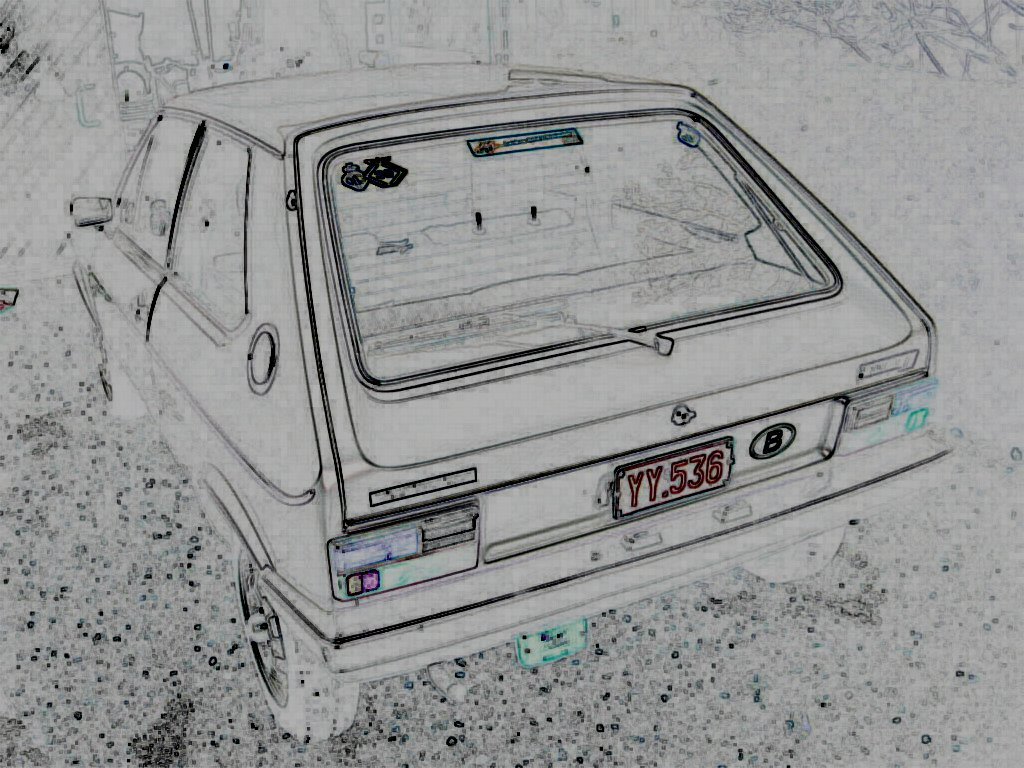
\includegraphics[width=0.5\textwidth]{YY536}
\end{center}
\end{oefening}

\begin{oefening}
We moeten 5 verschillende prijzen verloten onder de nummers 1 tot en met 100.
Na de trekking wordt elk nummer teruggelegd. Geef het aantal mogelijke
trekkingen.
\end{oefening}

\begin{oefening}
Op hoeveel manieren kunnen in een gezin met acht kinderen, de jongens en de
meisjes elkaar opvolgen ?
\end{oefening}

\begin{oefening}
Hoeveel getallen van 4 cijfers kan men vormen met de oneven cijfers ?
\end{oefening}

\begin{oefening}
Schrijf alle herhalingsvariaties op van de elementen a, b en c, twee aan twee
genomen.
Controleer het aantal.
\end{oefening}

\begin{oefening}
Op hoeveel manieren kunnen we een voetbalpronostiek invullen als er 13
wedstrijden worden gespeeld ?
\end{oefening}

\begin{oefening}
Hoeveel “woorden” kunnen we vormen met de letters \texttt{a, b, ..., k}. Elk woord
bestaat uit drie letters.
\end{oefening}

\begin{oefening}
Belgische nummerplaten bestaan uit 3 letters en 3 cijfers, bijvoorbeeld \texttt{ABA 123}. De letters \texttt{I} en de \texttt{O} worden niet gebruikt, wegens overeenkomsten met de 1 en de 0. Hoeveel mogelijkheden zijn er om nummerplaten samen te stellen.
\end{oefening}

\begin{oefening} % opmerking, geen herhalingsvariatie!
De fanfare kiest een nieuw bestuur. Uit de 20 leden wordt één directeur, één onderdirecteur en één secretaris gekozen. Op hoeveel manieren kan dit?
\end{oefening}

\begin{oefening}* % moeilijk
Hoeveel getallen bestaande uit 3 cijfers kunnen gemaakt worden met 3 vieren, 4 tweeën en 2 drieën.
\end{oefening}

\begin{oefening}*
Iedereen weet dat een trol 12 tanden heeft, 6 in elke kaak. Ooit was er eens een leger van 5000 trollen die een draak aanviel. Na het gevecht merkten de overlevende trollen dat geen twee van hun nog de zelfde verzameling tanden had (geen één trol had nog tanden op dezelfde plaats als een andere trol). Hoeveel trollen zijn er tijdens het gevecht tegen de draak op zijn minst gestorven?
\end{oefening}

\cleardoublepage
\section{Faculteiten}

\subsection{Definitie}

\paragraph*{n-faculteit}
\begin{mdframed}
\begin{align*}
\forall n \in \mathbb{N}\backslash\{0,1\}: n!&=n\cdot(n-1)\cdot(n-2)\cdot \cdots \cdot 3\cdot2\cdot1\\
                           1!&=1\\
                           0!&=1\\
\end{align*}
\end{mdframed}

\subsection{Berekenen met behulp van het rekentoetstel}

De toets voor $n$-faculteit bevindt zich boven het rechter haakje. Om bijvoorbeeld $24!$ uit te rekenen toetsen we
$$24 \zrm{SHIFT} \zrm{x!} \zrm{EXE}\;.$$

We krijgen een heel groot getal, namelijk $620448401733239439360000$. Voor de leesbaarheid zullen we deze grote getallen steeds in wetenschappelijke notatie schrijven. Dit wil zeggen dat de getallen zullen schrijven in de vorm $a \cdot 10^b$ met $1 \leq a < 10$ en met 2 cijfers na de komma. In ons geval schrijven we dus
\[24! = 6.20\EE{23}\]

\subsection{Eigenschap}

Bereken we de eerste faculteiten zonder \zrm{ZRM}
\begin{align*}
  2! &= 2 \cdot 1 = 2\\
  3! &= 3 \cdot 2 \cdot 1 = 6\\
  4! &= 4 \cdot 3 \cdot 2 \cdot 1 = 24\\
  5! &= 5 \cdot \underbrace{4 \cdot 3 \cdot 2 \cdot 1}_{=4!} = 5 \cdot 24 = 120
\end{align*}

Dan zien we snel dat er een manier is om faculteiten uit re rekenen als we reeds de waarde van de vorige faculteiten kennen. Daarom ook
\paragraph*{Eigenschap van de n-faculteit}
\begin{mdframed}
\begin{align*}
  (n+1)! &= (n+1) \cdot n!\\
  n!     &= n \cdot (n-1)!\\
\end{align*}
\end{mdframed}

\begin{oefening}
Als je weet dat
$$9!=362880\;.$$
Aan wat is dan $10!$ gelijk? Gebruik geen \zrm{ZRM}.
\end{oefening}

\begin{oefening}
Bereken zonder \zrm{ZRM}:
\begin{multicols}{3}
\begin{enumerate}[(a)]
  \itemsep.7em
  \item $\dfrac{17!}{14!}$
  \item $\dfrac{10!}{7!}$
  \item $\dfrac{11!}{8!}$
  \item $\dfrac{8!}{10!}$
  \item $\dfrac{3!\cdot 7!}{10!}$
  \item $\dfrac{12!-10!}{9!}$
\end{enumerate}
\end{multicols}
\end{oefening}

\begin{oefening}
Vereenvoudig:
\begin{multicols}{2}
\begin{enumerate}[(a)]
  \itemsep.7em
  \item $\dfrac{(n+1)!}{n!}$
  \item $\dfrac{(n-1)!}{n!}$
  \item $\dfrac{n!}{(n+1)!}$
  \item $\dfrac{(n+1)!}{(n-2)!}$
  \item $\dfrac{(n+2)!}{n!}$
  \item $\dfrac{(n+1)!}{n!}-\dfrac{n!}{(n-1)!}$
  \item $\dfrac{(n+1)!}{(n-1)!}-\dfrac{n!}{(n-2)!}$
  \item $\dfrac{n}{n!}$
\end{enumerate}
\end{multicols}
\end{oefening}

\begin{oefening}
Als je weet dat het getal $99!$ uit 156 cijfers bestaat, uit hoeveel cijfers bestaat dan het getal $100!$
\end{oefening}

\subsection*{Weetjes}
\begin{itemize}
  \item Zes weken is juist $10!$ seconden: ontbind $60\cdot 60\cdot 24\cdot 7\cdot 6$ in factoren en herschik en neem sommige factoren samen.
  \item Er zijn $52!=8.066\EE{67}$ manieren om een pak kaarten te schudden. Dit aantal is zo groot dat wanneer je een pak kaarten schudt, je eigenlijk zeker bent dat nog nooit iemand anders een pak in dezelfde volgorde geschud heeft!
  \item Men schat dat er ongeveer tussen de $10^{78}$ en $10^{82}$ atomen in het universum zijn. Kort kunnen we dus zeggen dat er ongeveer $60!$ atomen zijn.
\end{itemize}

\subsection{Formule voor $V^k_n$ met behulp van faculteiten}

We bereken $V^3_7$ door gebruik te maken van faculteiten:
\begin{align*}
  V^3_7 &= 7 \cdot 6 \cdot 5\\
        &= \dfrac{7 \cdot 6 \cdot 5 \, \color{gray}{ \cdot \, 4 \cdot 3 \cdot 2 \cdot 1}}{\color{gray}{4 \cdot 3 \cdot 2 \cdot 1}}\\
        &= \dfrac{7!}{4!}\\
        &= \dfrac{7!}{(7-3)!}\\
\end{align*}

We krijgen algemeen dan volgende formule

\paragraph*{Stelling}
\begin{mdframed}
$$V^k_n=\dfrac{n!}{(n-k)!}$$
\end{mdframed}

\paragraph*{Bewijs}
\begin{align*}
  V^k_n &= n \cdot (n-1) \cdot \ldots \cdot (n-k+1)\\
        &= \dfrac{n \cdot (n-1) \cdot \ldots \cdot (n-k+1) \, \color{gray}{ \cdot \, (n-k) \cdot (n-k-1) \cdot \ldots \cdot 1}}{\color{gray}{(n-k) \cdot (n-k-1) \cdot \ldots \cdot 1}}\\
        &= \dfrac{n!}{(n-k)!}\\
\end{align*}


\begin{oefening}
Om het aantal variaties van 20 elementen uit 24 elementen te berekenen hebben we twee formules:\\
\begin{itemize}
  \itemsep1em
  \item $\displaystyle V^{20}_{24}=24\cdot23\cdot22\cdot21\cdot\;\cdots\;\cdot(24-20+1)$
  \item $\displaystyle V^{20}_{24}=\dfrac{24!}{(24-20)!}$
\end{itemize}
\begin{enumerate}[(a)]
  \item Bereken op beide manieren het aantal variaties. Welke methode verkies je in dit geval?
  \item Doe hetzelfde voor het aantal variaties van 3 elementen uit 10 elementen. Welke methode verkies je in dit geval?
  \item Welke methode zou je kiezen als je het aantal variaties van 100 elementen uit 1000 elementen zou moeten berekenen? Het is niet nodig om dit te proberen, hiervoor is speciale software nodig want onze rekenmachines kunnen niet met zulke grote getallen overweg.
\end{enumerate}
\end{oefening}


\cleardoublepage
\section{Combinaties}

\subsection{Voorbeeld}

Op hoeveel manieren kunnen twee identieke bollen in vijf verschillende vakjes geplaatst worden? In elk vakje mag hoogstens één bol voorkomen.

We definiëren:
\begin{itemize}
  \item De bollen zijn identiek, we duiden één bol aan met de letter $B$
  \item De verzameling vakjes = $\{a, b, c, d, e\}$
\end{itemize}

We moeten twee gelijke bollen in vijf vakjes leggen. Dit is hetzelfde als: we moeten de twee bollen tegelijkertijd in de bakjes leggen. Vermits de 2 bollen identiek zijn heeft alléén het vakje belang waarin een bol ligt. De bol zelf speelt geen rol.

Een mogelijke plaatsing voor de bollen is dan
\[\ub[B]\ub\ub[B]\ub\ub\]

Deze plaatsing zouden we als een tweetal $(a, c)$ kunnen noteren. Maar elk tweetal, waarin dezelfde vakjes voorkomen zoals $(a, c)$ en $(c, a)$ stelt eenzelfde plaatsing voor.

De volgorde waarin de vakjes opgesomd worden heeft geen belang. We spreken nu af om de plaatsing te noteren als een verzameling waarin de elementen in alfabetische volgorde worden geschreven. De hierboven voorgestelde plaatsing wordt dan : $\{a, c\}$ en is een deelverzameling van de gegeven verzameling vakjes $\{a, b, c, d, e\}$.

Daar er bovendien in elk vakje hoogstens één bol ligt wordt geen enkel vakje herhaald. In een verzameling wordt óók geen element herhaald. Wel, de deelverzameling $\{a, c\}$, noemt men nu een combinatie zonder herhaling, kortweg combinatie, van 2 elementen gekozen uit 5 elementen.
Het aantal van zulke combinaties stellen we nu voor door het symbool $C^2_5$ en kunnen we als volgt bepalen:

Codeer het gegeven probleem als volgt: We kiezen 5 plaatsen, 2 ervan moeten gevuld worden met de letter $B$ van bol plaatsen, de overige drie moeten gevuld worden met de letter $L$ van leeg laten. Een voorbeeld is dan
\[\ub[B]\ub[L]\ub[B]\ub[L]\ub[L]\]

Dit is net hetzelfde probleem als we tevoor opgelost hebben met een wegenrooster! Eenvoudiger is om onmiddellijk de ondertussen gekende formule te gebruiken:
$$C^2_5 = \dfrac{5!}{2!\cdot (5-2)!} = 10$$

Let op de notatie : De $C$ is het symbool voor het aantal combinaties zonder herhaling. Het aantal beslissingen wordt als superscript (bovenaan) genoteerd. Het aantal vakjes (elementen) waar je keuze uit hebt wordt als subscript (onderaan) genoteerd.

\subsection{Formule}

\paragraph*{Combinaties}
\begin{mdframed}
Het aantal {\bf combinaties van $k$ elementen gekozen uit $n$ elementen} noteren we $C^k_n$ en er geldt:
$$C^k_n=\dfrac{n!}{k!\cdot(n-k)!}$$
\end{mdframed}

\paragraph*{Belangrijk}
\begin{itemize}
  \item Het maakt niet uit in welke volgorde dat de elementen worden gekozen, {\bf volgorde onbelangrijk}.
  \item Elk element kunnen we maar éénmaal kiezen, {\bf herhaling niet toegestaan}.
\end{itemize}

\subsection{Oefeningen}

\begin{oefening}
Voor het voetbalteam van de school stellen zich 19 leerlingen kandidaat.
\begin{enumerate}[(a)]
  \item Hoeveel elftallen kan de coach hiermee vormen?
  \item Bij het samenstellen van de ploeg voor een belangrijke wedstrijd wil de coach zijn vijf beste spelers zeker opstellen en zijn drie zwakste niet. Hoeveel ploegen kan hij nu vormen?
\end{enumerate}
\end{oefening}

\begin{oefening}
Een Belgische delegatie bestaat uit 7 Vlamingen en 5 Walen.
\begin{enumerate}[(a)]
  \item Hoeveel groepjes van 6 personen kan je hiermee vormen?
  \item Hoeveel groepjes bestaan uit 3 Vlamingen en 3 Walen?
\end{enumerate}
\end{oefening}

\begin{oefening}
Een firma heeft twee bedienden nodig (die hetzelfde werk moeten verrichten). Er zijn acht sollicitanten. Op hoeveel manieren kan de directie haar keuze bepalen?
\end{oefening}

\begin{oefening}
In een firma werken 15 arbeiders en 10 bedienden. Op hoeveel verschillende manieren kunnen we een comité samenstellen dat uit 3 arbeiders en 2 bedienden bestaat?
\end{oefening}

\begin{oefening}
Herinner je nog deze oefening uit het hoofdstuk van variaties:

{\em Op een boekenrek moeten 3 werken over wiskunde en 4 romans gerangschikt worden. We beschikken daartoe over 5 wiskundeboeken en over 6 romans. Op hoeveel manieren kunnen we de boeken rangschikken als ons opgelegd wordt de wiskundeboeken vooraan te plaatsen?}

Los deze nu opnieuw op, maar het is nu wel niet meer nodig om de wiskundeboeken vooraan te plaatsen.
\end{oefening}

\begin{oefening}
De bibliotheek bezit 15 verschillende werken van een schrijver die net de Nobelprijs voor literatuur heeft gekregen. Naar aanleiding daarvan worden 10 werken op een speciale tafel tentoongesteld. Hoeveel keuzemogelijkheden heeft de bibliothecaris?
\end{oefening}

\begin{oefening}
Bij vele spelletjes met een stel van 52 kaarten krijg je 13 kaarten.
\begin{enumerate}[(a)]
  \item Hoeveel mogelijkheden zijn er om uit 52 kaarten er 13 te trekken (zonder kaarten terug te leggen)?
  \item In hoeveel van die gevallen heb je geen enkele aas?
  \item Hoeveel mogelijkheden zijn er met schoppen aas?
  \item Hoeveel mogelijkheden zijn er met 4 azen?
  \item Hoeveel mogelijkheden zijn er met precies 3 azen?
  \item In hoeveel van die mogelijkheden heb je alle harten?
  \item Hoeveel mogelijkheden zijn er met 9 harten en 4 klaveren?
\end{enumerate}
\end{oefening}

\begin{oefening}
Bepaal voor de volgende problemen of het een combinatie of een variatie is.
\begin{enumerate}[(a)]
  \item Uit een klas worden zes leerlingen gekozen om een volleybalteam te vormen.
  \item Bij een verloting zijn drie prijzen te verdienen: een fiets, een fles wijn en een taart.
  \item Van 100 leraren van een school komen er vijf naar het schoolfeest.
  \item In een klas worden vijf kaartjes verloot voor een concert.
  \item Uit de muziek top 10 van vorige week stel je een persoonlijke top drie samen.
  \item Een vereniging kiest een voorzitter, een secretaris en een penningmeester.
  \item Een bondscoach kiest 24 spelers voor de selectie die hij meeneemt naar het WK.
\end{enumerate}
\end{oefening}

\begin{oefening}
Uit een selectie van 19 personen wordt een spelersraad van 6 spelers samengesteld. Hoeveel spelersraden zijn er mogelijk?
\end{oefening}

\begin{oefening}
Uit de spelersraad van 6 personen wordt een bestuur gekozen dat bestaat uit een voorzitter, een secretaris en een penningmeester. Hoeveel besturen zijn er mogelijk?
\end{oefening}

\begin{oefening}
Uit de selectie van 19 personen wordt een feestcommissie gekozen die uit 5 personen bestaat. Hoeveel feestcommissies zijn er mogelijk?
\end{oefening}

\begin{oefening}
In de mediatheek staat 14 CD's met klassieke muziek en 12 CD's met popmuziek. Margo kiest 5 CD's met klassieke muziek. Hoeveel mogelijkheden zijn er?
\end{oefening}

\begin{oefening}
Joni gooit 13 keer met een geldstuk. Telkens noteert hij K(op) en M(unt). Zo ontstaat een serie met 13 letters K en M.
\begin{enumerate}[(a)]
  \item Hoeveel series zijn er met 11 keer K?
  \item Hoeveel series zijn er met 9 keer een M?
  \item Hoeveel series zijn er die met K beginnen en met M eindigen?
\end{enumerate}
\end{oefening}

\cleardoublepage
\section{Gemengde oefeningen}

\subsection{Reeks 1}

\begin{oefening}
Het probleem kan herschreven worden met {\em \small (Schrappen wat niet past.)}
\begin{itemize}
  \item {\bf EN} $\Rightarrow$ productregel/somregel.
  \item {\bf OF} $\Rightarrow$ productregel/somregel.
\end{itemize}
\end{oefening}

\begin{oefening}
Vul volgende schema aan met
\begin{itemize}
  \item Variatie van $k$ elementen uit $n$ elementen
  \item Permutatie van $n$
  \item Herhalingsvariatie van $k$ elementen uit $n$ elementen
  \item Combinatie van $k$ elementen uit $n$ elementen
\end{itemize}
\begin{center}
  \begin{tabular}{|c|c|c|}
  \hline
                        & Zonder herhaling & Met herhaling \\
  \hline
  Volgorde belangrijk   & \hspace*{4cm}    & \hspace*{4cm} \\[2cm]
  \hline
  Volgorde onbelangrijk &                  &               \\[2cm]
  \hline
  \end{tabular}
\end{center}
\end{oefening}

\begin{oefening}
Men gooit twee verschillende muntstukken op. Hoeveel mogelijke uitkomsten zijn er?\\
{\em Hint: aangezien de muntstukken verschillend zijn, moeten we rekening houden met de volgorde.}
\end{oefening}

\begin{oefening}
Hoeveel getallen van vier cijfers kan men vormen door uitsluitend de cijfers 2, 4 en 6 te gebruiken?\\
{\em Hint: probeer dit probleem grafisch voor te stellen.}
\end{oefening}

\begin{oefening}
Toon aan: $$(n+2)!-(n+2)n!=n(n+2)n!\;.$$
{\em Hint: maak gebruik van het feit dat $(n+1)!=(n+1)n!$ en dus $(n+2)!=(n+2)(n+1)n!$ is.}
\end{oefening}

\begin{oefening}
Op een boekenplank moeten we 5 boeken over fysica en 2 boeken over chemie rangschikken. We beschikken over 8 fysicaboeken en 6 chemieboeken. Op hoeveel manieren is het rangschikken mogelijk als de fysicaboeken steeds vooraan moeten staan?\\
{\em Hint: pak eerst het probleem over de fysicaboeken aan, daarna het probleem over de chemie boeken. Aangezien je zowel de fysicaboeken als de chemieboeken moet plaatsen moet je daarna de productregel toepassen.}
\end{oefening}

\begin{oefening}
We beschikken over de letters $b$, $a$, $r$, $s$, $t$. We gaan hiermee 'woorden' vormen van vier verschillende letters. Deze woorden moeten geen betekenis hebben en ook niet uitspreekbaar zijn.
\begin{enumerate}[(a)]
  \item Hoeveel woorden kan men vormen?
  \item Hoeveel daaronder beginnen met een $b$?\\
  {\em Hint: Wat weet je al zeker over de eerste letter?}
  \item Hoeveel eindigen op $st$?
  \item Hoeveel daarvan bevatten de $r$?\\
  {\em Hint: Hoeveel woorden zijn er in het totaal, welke woorden zijn daaruit slecht?}
\end{enumerate}
\end{oefening}

\begin{oefening}
\begin{enumerate}[(a)]
  \item Op hoeveel manieren kan men zes verschillende boeken rangschikken?
  \item Hoeveel manieren zijn er nog als een bepaald boek {\em niet} op de eerste plaats mag komen?
\end{enumerate}

\end{oefening}

\begin{oefening}
Op hoeveel manieren kan men vijf personen naast elkaar aan een ronde tafel plaatsen? Niet de plaats waar men zit, maar de positie t.o.v. de andere is belangrijk.
\end{oefening}

\begin{oefening}
Hoeveel diagonalen heeft een convexe zeshoek? Een veelhoek is convex als hij geen interne hoeken heeft die groter zijn dan $180^\circ$.
\end{oefening}

\begin{oefening}
Op hoeveel manieren kan men vijf verschillende brieven naar drie verschillende bestemmelingen sturen?
\end{oefening}

\begin{oefening}
Het codewoord van een kluis bestaat uit drie letters. Om een “woord” te vormen en de juistheid
ervan na te gaan heeft men 15 sec nodig. De “kraker” slaagt pas in de allerlaatste poging om
de goede combinatie te ontdekken. Hoeveel tijd had hij hier voor nodig?
\end{oefening}

\begin{oefening}
In de mediatheek staat 14 CD's met klassieke muziek en 12 CD's met popmuziek. Wout kiest 8 CD's met popmuziek. Hoeveel mogelijkheden zijn er?
\end{oefening}

\begin{oefening}
Voor een toelatingstest moeten 16 tweekeuzevragen worden beantwoord.
\begin{enumerate}[(a)]
  \item Hoeveel mogelijkheden zijn er in totaal om het formulier in te vullen?
  \item Hoeveel mogelijkheden zijn er met 11 juiste antwoorden?
  \item Hoeveel mogelijkheden zijn er met meer dan 13 juiste antwoorden?
  \item Hoeveel mogelijkheden zijn er met minder dan 3 juiste antwoorden?
\end{enumerate}
\end{oefening}

\begin{oefening}
 Winkelier Phillips heeft zijn etalage versierd met feestverlichting. De verlichting bestaat uit 16 lampjes die onafhankelijk van elkaar voortdurend aan en uit gaan. Een mogelijke situatie is dat de lampjes 2, 5, 7, 9, 10 en 12 branden.
\begin{enumerate}[(a)]
  \item Hoeveel situaties zijn er in totaal mogelijk?
  \item In hoeveel situaties branden er precies 4 lampjes?
  \item In hoeveel situaties branden er meer dan 13 lampjes?
  \item In hoeveel situaties branden in ieder geval het eerste en de laatste twee lampjes?
\end{enumerate}
\end{oefening}

\begin{oefening}
Er zijn 10 kandidaten in een quiz (A, B, C, D, E, F, G, H, I, J). Drie van deze mensen mogen aan de finale meedoen, bijvoorbeeld D, J en B. Hoeveel mogelijkheden zijn er voor de finalisten?
\end{oefening}

\begin{oefening}
Er staan 7 boeken in de kast: K, L, M, N, O, P en Q. In de kerstvakantie lees ik één van deze boeken, daarna nog één en daarna nog één (nooit twee keer dezelfde natuurlijk). Bijvoorbeeld: eerst P, dan K, dan M. Hoeveel van zulke mogelijkheden zijn er?
\end{oefening}

\begin{oefening}
In een kamer hangen 5 TL-buizen. Twee hiervan branden. Hoeveel mogelijkheden zijn er?
\end{oefening}

\begin{oefening}
Van 20 koeien worden er 4 geslacht. Hoeveel mogelijkheden zijn er?
\end{oefening}

\begin{oefening}
Uit een groep van 8 mensen worden 2 mensen gekozen. Eentje om de zaal te versieren, eentje om de geluidsapparatuur aan te sluiten (bijvoorbeeld Jan voor de versiering, Kees voor de geluidsapparatuur). Hoeveel mogelijkheden zijn er?
\end{oefening}

\begin{oefening}
Een muziekband heeft een repertoire van 10 liedjes. Voor een optreden mogen ze drie liedjes uitkiezen. Hoeveel mogelijkheden zijn er voor die keuze?
\end{oefening}

\pagebreak
\subsection{Reeks 2}

\begin{oefening}
We willen een wachtwoord maken dat bestaat uit 4 verschillende cijfers. Hoeveel verschillende
mogelijkheden zijn er als we cijfers kiezen uit $\{0,1,2,3,4,5,6,7,8,9\}$.
\end{oefening}

\begin{oefening}
Een goochelaar heeft momenteel 25 trucjes onder de knie. Bij een optreden moet hij 6 trucjes
‘opvoeren’. Op hoeveel manieren kan hij zijn keuze maken?
\end{oefening}

\begin{oefening}
In een klas zitten 9 leerlingen die na elkaar een mondeling examen moeten afleggen.
Op hoeveel verschillende manieren kan de leerkracht een rooster opstellen met de
volgorde waarin de leerlingen moeten komen?
\end{oefening}

\begin{oefening}
Tijdens de les aardrijkskunde maken de leerlingen kennis met enkele vlaggen. Ze mogen zelf
vlaggen (ook fictieve) inkleuren, maar de vlaggen moeten wel bestaan uit drie horizontale banen met
elk een verschillende kleur. De leerlingen beschikken over 8 verschillende kleuren. Hoeveel vlaggen
kan men samenstellen?
\end{oefening}

\begin{oefening}
2000 atleten lopen de marathon van Brussel. Hoeveel mogelijke uitslagen bestaan er?
{\em Opgelet: Uitrekenen is hier niet nodig, het is voldoende als je de formule geeft!}
\end{oefening}

\begin{oefening}
In een klas staan 10 stoelen. Op hoeveel verschillende manieren kunnen acht leerlingen van een
klas plaatsnemen?
\end{oefening}

\begin{oefening}
Hoeveel verschillende woorden (ook woorden zonder betekenis) kunnen we vormen met alle zeven
letters van het woord \verb#AVELGEM#?
\end{oefening}

\begin{oefening}
Uit een klas van zestien leerlingen moeten twee leerlingen gekozen worden die zullen zetelen in de
leerlingenraad. Hoeveel mogelijkheden zijn er?
\end{oefening}

\begin{oefening}
Albert, Bo, Colette en Diana zijn 4 leden uit het bestuur van een ‘wiskundeclub’. Onder hen moet
men een voorzitter, ondervoorzitter en penningmeester kiezen. Op hoeveel manier kan dit?
\end{oefening}

\begin{oefening}
Een voetbalclub biedt de mogelijkheid om zelf een abonnement van vijf
thuiswedstrijden samen te stellen uit een aanbod van 15 thuiswedstrijden die de
ploeg speelt. Hoeveel mogelijkheden zijn er?
\end{oefening}

\begin{oefening}
Aan een formule 1-wedstrijd nemen twintig autopiloten deel. Er wordt gevraagd de eerste 5
autopiloten in de juiste volgorde te voorspellen. Hoeveel van dergelijke voorspellingen zijn er
mogelijk?
\end{oefening}

\begin{oefening}
In een klas zitten 5 jongens en 9 meisjes. Er moet een delegatie gekozen worden. Op hoeveel
manieren kan dit als...
\begin{enumerate}[(a)]
  \item we 3 willekeurige leerlingen kiezen?
  \item we 2 jongens en 4 meisjes moeten kiezen
  \item er één jongen en 7 meisjes moeten gekozen worden.
\end{enumerate}
\end{oefening}

\begin{oefening}
Met de cijfers 1 tem. 9 vormen we getallen van 6 verschillende cijfers.
\begin{enumerate}[(a)]
  \item Hoeveel getallen kunnen we zo vormen?
  \item Hoeveel van deze getallen beginnen niet met 9?
  \item Hoeveel ervan beginnen niet met 12?
\end{enumerate}
\end{oefening}

\begin{oefening}
Op hoeveel manieren kan één vak van een lottoformulier ingevuld worden? (hierbij
moeten 6 cijfers aangeduid worden van 1 tot en met 42)
\end{oefening}

\begin{oefening}
Acht vrienden gaan samen tennissen.
\begin{enumerate}[(a)]
  \item Hoeveel verschillende partijen enkelspel kunnen ze spelen?
  \item Hoeveel verschillende partijen dubbelspel kunnen ze spelen?
\end{enumerate}
\end{oefening}

\begin{oefening}
In een klas staan 5 stoelen voor 5 leerlingen. Op hoeveel manieren kunnen we de
leerlingen laten plaatsnemen?
\end{oefening}

\begin{oefening}
Tijdens de vakantie wil ik graag een vakantiejob doen. Er zijn echter nog 5 andere
kandidaten voor deze job. Uiteindelijk zullen er twee studenten aangenomen worden.
Hoeveel mogelijkheden heeft de baas van het bedrijf om deze studenten te bepalen?
\end{oefening}

\begin{oefening}
Op hoeveel manieren kunnen we paswoorden maken van 5 cijfers als we mogen kiezen uit
$\{1,2,3,4,5,6,7,8,9\}$?
\end{oefening}

\begin{oefening}
De spelerskern van een voetbalploeg bestaat uit 3 doelmannen, 9 verdedigers, 7
middenvelders en 5 spitsen. Men wil een soort raad samenstellen die zal
onderhandelen over winstpremies bij eindrondewedstrijden enz...Deze raad bestaat
uit 2 doelmannen, 2 verdedigers, 2 middenvelders en 2 spitsen. Op hoeveel
verschillende manieren kan deze raad samengesteld worden?
\end{oefening}

\begin{oefening}
Op een receptie zijn 50 mensen uitgenodigd. Iedereen geeft elkaar de hand. Hoeveel handen worden
er dan geschud?
\end{oefening}

\begin{oefening}
Hoeveel woorden van 9 letters kan men vormen als de eerste 5 letters medeklinkers moeten zijn en
de laatste 4 klinkers?
\end{oefening}

\begin{oefening}
De pincode voor het toestel dat elektronisch bankieren toelaat, bestaat uit 4 cijfers.
\begin{enumerate}[(a)]
  \item Hoeveel codes zijn er mogelijk?
  \item Hoeveel codes met 4 verschillende cijfers zijn er mogelijk?
  \item Hoeveel codes bevatten het cijfer 5?
\end{enumerate}
\end{oefening}

\begin{oefening}
Hoeveel verschillende sommen kan men bekomen als men drie van de getallen 1, 10, 100, 1000,
10000 en 100000 optelt?
\end{oefening}

\begin{oefening}
In een voetbalcompetitie zijn er 18 ploegen die elk tweemaal tegen elkaar spelen (1 maal thuis en 1 maal op
verplaatsing ). Hoeveel wedstrijden worden er gespeeld?
\end{oefening}

\end{document}
